\chapter{Optimalization}

This chapter is named optimalization due to its contents; here we will account for the choices we compose to optimize a potential machine learning algorithm. Initially, that involves finding what information is stored within the databases and the compromise of gathering the information, which further evolves into finding optimal hyperparameters for each approach.

\begin{comment}
\section{Time of extraction and featurization}

The initial thought behind

\begin{table}[!ht]
\centering
\caption{}
\label{tab:timing-extraction}
\noindent\makebox[\textwidth]{
\begin{tabular}{M{3.0cm} M{4.0cm} M{4.0cm}}
  \hline
  \hline
  Database & Extraction period & Estimated time usage  \\
  \hline
  Materials Project & December $2020$ & $5$ min \\
  Citrine Informatics & December $2020$ & $2$ min  \\
  OQMD & December $2020$ & $3$ min \\
  AFLOW & January $2020$ - February $2021$ & $17$ days \\
  AFLOW-ML & January $2020$ - February $2021$ & $16$ days \\
  JARVIS-DFT & January $2020$ & $5$ min \\
  \hline
  \hline
\end{tabular}
}
\end{table}

\end{comment}
% 139.367, icsd: 52.116, bg: 68141
The first step of this work was to find data from Materials Project, involving entries that are associated with an ICSD structure and have a PBE-GGA calculated band gap of minimum $0.1$eV. Out of $126.335$ existing entries in Materials Project, $48.644$ ($39\%$) were found to have an associated ICSD-structure, while $65.783$ ($52\%$) materials had a calculated band gap of at least $0.1$eV. It was found that $25271$ ($20\%$) materials have the band gap minimum and an associated ICSD-structure. It should be noted that these numbers are based on data extraction in December of $2020$, while the extraction from other databases and featurization related to this work was done in the time period of December $2020$ to March $2021$. In February of $2021$, over $30.000$ new materials were added in a large update\footnote{https://matsci.org/t/materials-project-database-release-log/1609/16 23.04.2021}. These new entries are not included in this work, and therefore the number of entries in our Materials Project are based on the latest release in $2020$, which is named V2020.09.08.%, however there are present more than than $2000$ new entries that satisfy the initial MP requirement now.

Two visualizations of two different distributions of the data is found in figure \ref{fig:hist_ox} and \ref{fig:hist_bg}. The first figure visualize the distribution of oxid types as a function of compound type, and reveal that the majority of compounds are either binary, ternary, quaternary or quinary, where the majority of the materials are either oxide or not. This is important to know considering our labelling approaches, in particular the insightful approach where we handpicked good entries. None of the entries labelled as good candidates were oxides, which means that potentially half of the the test set could potentially be considering as bad candidates by the models.

\clearpage

\begin{figure}
      \centering
      \includegraphics{../predicting-solid-state-qubit-candidates/reports/figures/buildingFeatures/histogram_oxid_nelements.pdf}
      \vspace*{-130mm}
      \caption{Distribution of oxid types as a function of number of elements in compounds in the data. The majority of the entries are found as oxides, while the second most frequent type is not an oxid. }
      \label{fig:hist_ox}
\end{figure}

\begin{figure}
      \centering
      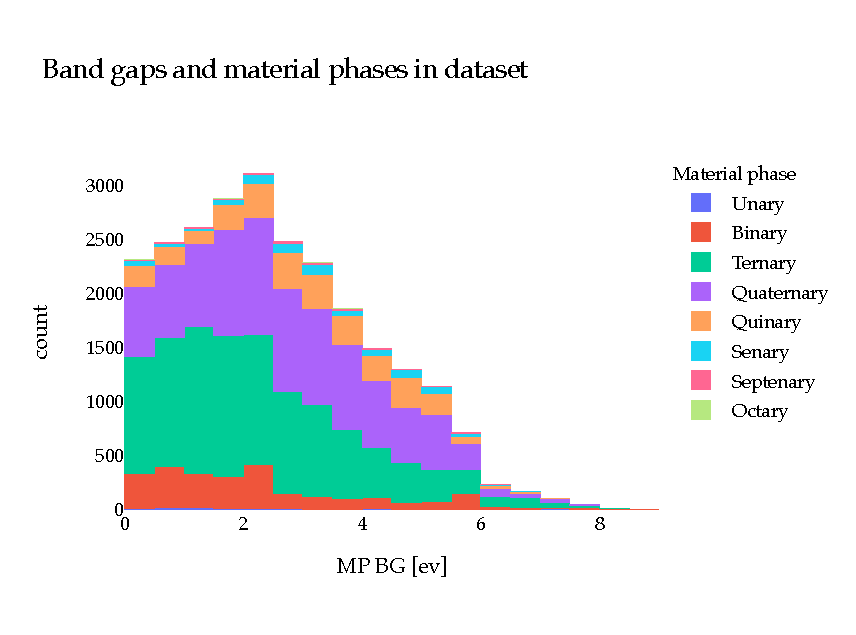
\includegraphics{../predicting-solid-state-qubit-candidates/reports/figures/buildingFeatures/histogram_bg_nelements.pdf}
      \vspace*{-130mm}
      \caption{Distribution of band gaps as function of compound type in the data. The majority of compounds are ternary and quaternary, while the simpler compounds are few.}
      \label{fig:hist_bg}
\end{figure}

\clearpage

\noindent The second figure visualize the compound type as function of band gap, as calculated by Materials Project. Most of the materials existing in the data has a band gap lower than $2.3$eV, where ternary compounds are most prominent. For larger values, we observe that quaternary compounds becomes dominant for larger values.

\section{Comparing functionals for band gaps}

Since the true size of a band gap can not be accurately determined by ab-initio calculations, we provide information regarding five different methods to obtain band gaps as visualized in figure \ref{fig:band gaps}. We have extracted experimental band gaps from Citrine Informatics that match the entries made by the initial MP query, involving entries that are associated with an ICSD structure that have a PBE-GGA calculated band gaps of minimum $0.1$. All the band gaps to the left are found common with all databases through screening of correct structure, space group and ICSD-ID, while the figures to the right are only compared to the experimental database of Citrine Informatics. We found it helpful with the ICSD-tag to find similarities due to databases often have different norms and data-structures of descriptors, which proves challenging for comparison of stored calculations. If we were to exclude ICSD-tags, it would result in a much larger foundation to find similar entries, however, we found that the determination of similar entries would experience a large deviation when it comes to structures. By including an ICSD-tag, we reduce the basis of comparison but find more than $98\%$ identical space group for entries in each database compared to Materials Project.

It was found that a very small portion of the data extracted from AFLOW was associated with an ICSD-tag, only $5$ similar entries to the other databases, and therefore we have excluded the database from further consideration.

In the figures of \ref{fig:band gaps}, we observe each entry marked as black or blue dots. The dotted lines visualize the optimal ratio of estimated band gap to experimental values, while the red lines shows an linear least square fit to the data with the scrabbled area being the $95\%$ confidence interval. The data that constitute the left figures are based on $82$ similar entries, while the right figures constitute of more entries depending on the respective database. The data restriction was due to a small experimental database.

Initally, we wanted to include the right figures in the attempt of reducing the confidence interval with increasing the data points, but instead we find that the uncertainty of the confidence interval increase for all ab-initio calculations. This is due to the fact that the majority of the new entries are found for low band gap values, where the mismatch between experimental and calculated values are the largest. The discrepency seems to be largest for values under $5$eV, where entries are either calculated to have a very large band gap where the experimental values report a very low band gap, which is also true the opposite case. One reason for this is that we have no information regarding the experiment where the band gap was determined. The information we from the experimental database is only considered the chemical formula of a compound, whereas the structure or ICSD-entry remains unknown. However, the same data of experimental values have been considered through other articles \cite{Ward2018, Ferrenti2020}.

Therefore, we find that the functional applied for Materials Project are found to underestimate the band gap with $30-60\%$ while OQMD underestimates the band gap by $25-55\%$. AFLOW-ML also severily underestimates the band gap by $30-60\%$, but additionally have problems to accurately predict if a material is a metal or not. Many materials with both experimental and ab-initio calculations that showed a band gap of more than $1$eV was predicted as metals by AFLOW-ML. JARVIS-DFT, on the other hand, was found to underestimate the band gap by $20-60\%$ for the OptB88 and $0-30\%$ for TB-mBJ functionals.



%Similar to the results of \citeauthor{Ferrenti2020} \cite{Ferrenti2020}, we find

\clearpage
\begin{figure}[ht!]
    \centering
    \begin{subfigure}[t]{1\textwidth}
        \centering
        \input{../predicting-solid-state-qubit-candidates/reports/figures/bandgaps/mp.tex}
        \caption{}
    \end{subfigure}%

    \begin{subfigure}[t]{1\textwidth}
        \centering
        \input{../predicting-solid-state-qubit-candidates/reports/figures/bandgaps/oqmd.tex}
        \caption{}
    \end{subfigure}

    \begin{subfigure}[t]{1\textwidth}
        \centering
        \input{../predicting-solid-state-qubit-candidates/reports/figures/bandgaps/aflowml.tex}
        \caption{}
    \end{subfigure}
\end{figure}

\begin{figure}[t!]\ContinuedFloat
    \centering
    \begin{subfigure}[t]{1\textwidth}
        \centering
        \input{../predicting-solid-state-qubit-candidates/reports/figures/bandgaps/jarvis_tbmbj.tex}
        \caption{}
    \end{subfigure}%

    \begin{subfigure}[t]{1\textwidth}
        \centering
        \input{../predicting-solid-state-qubit-candidates/reports/figures/bandgaps/jarvis_opt.tex}
        \caption{}
    \end{subfigure}
    \vspace*{-130mm}
    \caption{Comparison of reported experimental band gaps to those calculated by (a) Materials Project, (b) Open Quantum Materials Database, (c) AFLOW-ML, (d) JARVIS-DFT (TB-mBJ) and (e) JARVIS-DFT (OptB88). The figures to the left show reported band gaps that have been found to be common through all databases, while the figures to the right are only common with experimentally reported values from Citrine Informatics. All entries have been extracted in the period of january to march of $2021$. }
    \label{fig:band gaps}
\end{figure}

\clearpage

\section{Technical details on ML classifiers}

%In this section we will provide technical details on the classifiers considering the training process. For each approach, we will apply combinations of principal components ranging from just one to several and look at the resulting implications. For each approach we can end up with over twenty different optimalization processes, which in total could potentially result in over sixty  in total. Therefore, we will not make an extensive analysis for every model, but emphasis important distinctions between the models and provide background for principal choices made. However, it should be noted that an an extensive automated analysis is distributed through the MIT license at the Github repository \textit{predicting-solid-state-qubit-candidates} \cite{Ohebbi2021}.

In the evaluation of the approaches, we apply a $5\times 5$ stratified cross-validation when iterating through the hyperparameter combinations. For random forest, gradient boost and decision tree, we found that by adjusting the parameters responded to severe overfitting except for the default values defined by Scikit-learn. The only parameter that we found could potentially improve the evaluation metric $f1$ was maximum number of depth for the trees grown, which we adjusted between $1$ and $8$. For logistic regression, we choose to adjust the regulariation strength with seven logaritmical adjusted values $10^{-3}$ to $10^{5}$, and use either $200$ or $400$ iterations to reach convergence.

When searching for the optimal number of principal components, we iterated over every odd number of principal components from $1$ to the upper restricted number which defines an accumulated variance of $95\%$ from the principal component analysis. Due to the large number of principal components, we end up fitting $25$ folds for each of $1232$ parameter combinations, totalling up to $30800$ individual models, just for logistic regression for one approach. This serves as an additional motivator to keep the models simple, and accordingly shows how easy an initial complex step might evolve into an unfeasible amount of information. Therefore, we will not make an extensive analysis for every model, but emphasis important distinctions between the general models and provide background for principal choices made. However, it should be noted that a larger automated analysis is distributed through the MIT license at the Github repository \textit{predicting-solid-state-qubit-candidates} \cite{Ohebbi2021}.

\subsection{The Ferrenti approach}

We visualize the grid search for the optimal number of principal components in figure \ref{fig:01-pca}, where we present the mean training score, mean test score and mean f1 score as a function of principal components used in the models. For each principal component, we visualize the optimal combination of hyperparameters based on the f1-score in the model. Common to all models is the improvement of scores up to around $50$ principal components, where random forest and the decision tree slowly starts to overfit. From figure \ref{fig:q1-DT}, we see that the metrics gets heavily effected for larger values of principal components except for decision trees. We can observe that the f1-score is not varying as much as the other metrics due to an increasing number of positive predictions. This means that the accuracy of positive predictions are dominating the overall accuracy measurement, and we would expect a large amount of training data being predicted as positive candidates. Similar to decision trees are random forest, which also show sign of overfitting for larger values of principal components. However, as a result of several weak trees, it show smaller signs of overfitting than the indications seen by the decision tree algorithm.

Gradient boost, on the other hand, experience minor changes for larger number of principal components, where the automated optimal component marked could easily be $50$ principal components less without any remarks to the models metrics. We find that by using only a few principal components will make it reach almost $100\%$ training accuracy, but does not show any sign on overfitting.

In \ref{tab:01-pc}, we find the precise measurements for each evaluation metric for the optimal number of principal components, which is visualized as dotted lines in figure \ref{fig:01-pca}. We find that the best performing model is logistic regression, but is dependent on a large amount of principal components. Random forest and gradient boost perform comparably, with and f1 score of $0.93$ and $0.95$, respectively.  %Yet, with almost a $100\%$ score in both test and f1, the model is perhaps overfitted. Decision trees scores an $f1$ score of $0.84$, but

%Logistic regression, in figure \ref{fig:q1-DT}, improves all metrics and does perform overall best according to the metrics.


\begin{figure}[ht!]
  \begin{subfigure}[b]{0.5\textwidth}
    \input{../predicting-solid-state-qubit-candidates/reports/figures/pca-scores/01-ferrenti-approach-176-LOG-final.tex}
    \caption{}
    \label{fig:q1-LOG}
  \end{subfigure}%
  \hfill
  \begin{subfigure}[b]{0.5\textwidth}
    \input{../predicting-solid-state-qubit-candidates/reports/figures/pca-scores/01-ferrenti-approach-176-DT-final.tex}
    \caption{}
    \label{fig:q1-DT}
  \end{subfigure}

  \begin{subfigure}[b]{0.5\textwidth}
    \input{../predicting-solid-state-qubit-candidates/reports/figures/pca-scores/01-ferrenti-approach-176-RF-final.tex}
    \caption{}
    \label{fig:q1-RF}
  \end{subfigure}%
  \hfill
  \begin{subfigure}[b]{0.5\textwidth}
    \input{../predicting-solid-state-qubit-candidates/reports/figures/pca-scores/01-ferrenti-approach-176-GB-final.tex}
    \caption{}
    \label{fig:q1-GB}
  \end{subfigure}
  \vspace*{-130mm}
  \caption{{Four visualizations for each model of the grid-search with the resulting optimal number of principal compoonents through a $5\times 5$ stratified cross-validation. The upper limit of principal components is decided by the explained accumulated variance at $95\%$, while the optimal model is found by using the $f1$ score. The specific scores for the arbitrary number of principal components is found in the Appendix \ref{appendix:Optimalization}.}}
  \label{fig:01-pca}
\end{figure}


\begin{table}[!ht]
\centering
\caption{Table }
\label{tab:01-pc}
\noindent\makebox[\textwidth]{
\begin{tabular}{M{2.0cm} M{3.0cm} M{3.0cm} M{3.0cm} }
  \hline
  \hline
   Model & Optimal number of PC & Mean (std) test score &  Mean (std) f1-score \\
  \hline
  LOG & 173 & $0.98(0.008)$ & $ 0.99(0.006)$ \\
  DT & 37 & $0.79(0.024)$ & $ 0.84(0.020)$ \\
  RF & 50 & $0.90(0.020)$  & $ 0.93(0.014)$ \\
  GB & 104 & $0.93(0.014)$ & $ 0.95(0.010)$ \\
  \hline
\end{tabular}
}
\end{table}

\begin{comment}
\begin{figure}[!tbp]
  \begin{subfigure}[b]{0.5\textwidth}
    \include{../predicting-solid-state-qubit-candidates/reports/figures/pca-scores/01-ferrenti-approach-5-RF.pgf}
    \caption{}
    \label{fig:q1-GB}
  \end{subfigure}%
  \hfill
  \begin{subfigure}[b]{0.5\textwidth}
    \include{../predicting-solid-state-qubit-candidates/reports/figures/pca-scores/01-ferrenti-approach-5-GB.pgf}
    \caption{}
    \label{fig:q1-RF}
  \end{subfigure}

  \begin{subfigure}[b]{0.5\textwidth}
    \include{../predicting-solid-state-qubit-candidates/reports/figures/pca-scores/01-ferrenti-approach-5-DT.pgf}
    \caption{}
    \label{fig:q1-DT}
  \end{subfigure}%
  \hfill
  \begin{subfigure}[b]{0.5\textwidth}
    \include{../predicting-solid-state-qubit-candidates/reports/figures/pca-scores/01-ferrenti-approach-5-LOG.pgf}
    \caption{}
    \label{fig:q1-LOG}
  \end{subfigure}
  \vspace*{-95mm}
  \caption{{Four figures displaying hyperparameter search for the first approach. The best estimator is visualized for all hyperparameters as a function of principal components during a grid search with a 5x5 stratified cross validation. The lower plots visualizes the explained variance ratio, both accumulated and stepwise. The dotted lines marks the optimal hyperparameter-combination, while the error bars display the standard deviation. }}
\end{figure}
\end{comment}

\clearpage

\subsection{The augmented Ferrenti approach}

\begin{figure}[!tbp]
  \begin{subfigure}[b]{0.5\textwidth}
    \includegraphics[width=\textwidth]{../predicting-solid-state-qubit-candidates/reports/figures/pca-scores/02-determined-approach-5-RF\space.pdf}
    \caption{}
    \label{fig:q2-GB}
  \end{subfigure}%
  \hfill
  \begin{subfigure}[b]{0.5\textwidth}
    \includegraphics[width=\textwidth]{../predicting-solid-state-qubit-candidates/reports/figures/pca-scores/02-determined-approach-5-GB\space.pdf}
    \caption{}
    \label{fig:q2-RF}
  \end{subfigure}

  \begin{subfigure}[b]{0.5\textwidth}
    \includegraphics[width=\textwidth]{../predicting-solid-state-qubit-candidates/reports/figures/pca-scores/02-determined-approach-5-DT\space.pdf}
    \caption{}
    \label{fig:q2-DT}
  \end{subfigure}%
  \hfill
  \begin{subfigure}[b]{0.5\textwidth}
    \includegraphics[width=\textwidth]{../predicting-solid-state-qubit-candidates/reports/figures/pca-scores/02-determined-approach-5-LOG\space.pdf}
    \caption{}
    \label{fig:q2-LOG}
  \end{subfigure}
  \vspace*{-95mm}
  \caption{{Four figures displaying hyperparameter search for the second approach. The best estimator is visualized for all hyperparameters as a function of principal components during a grid search with a 5x5 stratified cross validation. The lower plots visualizes the explained variance ratio, both accumulated and stepwise. The dotted lines marks the optimal hyperparameter-combination, while the error bars display the standard deviation. }}
\end{figure}

\clearpage

\subsection{The insightful approach}



\begin{figure}[ht!]
  \begin{subfigure}[b]{1.0\textwidth}
    \centering
    \input{../predicting-solid-state-qubit-candidates/reports/figures/pca-scores/03-insightful-approach-176-label.tex}
  \end{subfigure}
  \begin{subfigure}[b]{0.5\textwidth}
    \input{../predicting-solid-state-qubit-candidates/reports/figures/pca-scores/03-insightful-approach-176-LOG.tex}
    \caption{}
    \label{fig:q3-LOG}
  \end{subfigure}%
  \hfill
  \begin{subfigure}[b]{0.5\textwidth}
    \input{../predicting-solid-state-qubit-candidates/reports/figures/pca-scores/03-insightful-approach-176-DT.tex}
    \caption{}
    \label{fig:q3-DT}
  \end{subfigure}
  \begin{subfigure}[b]{0.5\textwidth}
    \input{../predicting-solid-state-qubit-candidates/reports/figures/pca-scores/03-insightful-approach-176-RF.tex}
    \caption{}
    \label{fig:q3-RF}
  \end{subfigure}%
  \hfill
  \begin{subfigure}[b]{0.5\textwidth}
    \input{../predicting-solid-state-qubit-candidates/reports/figures/pca-scores/03-insightful-approach-176-GB.tex}
    \caption{}
    \label{fig:q3-GB}
  \end{subfigure}

  \vspace*{-130mm}
  \caption{{Four visualizations for each model of the grid-search with the resulting optimal number of principal compoonents through a $5\times 5$ stratified cross-validation. The upper limit of principal components is decided by the explained accumulated variance at $95\%$, while the optimal model is found using the $f1$ score.}}
  \label{fig:03-pca}
\end{figure}


\begin{table}[!ht]
\centering
\caption{Table }
\label{tab:03-pc}
\noindent\makebox[\textwidth]{
\begin{tabular}{M{2.0cm} M{3.0cm} M{3.0cm} M{3.0cm}M{3.0cm}M{3.0cm} }
  \hline
  \hline
   Model & PC & Mean test &  Mean recall & Mean precision & mean f1\\
  \hline
  LOG & $129$ & $0.96(0.018)$ & $0.96(0.036)$ & $0.93(0.041)$ & $0.94(0.025)$ \\
  DT & $3$    & $0.94(0.025)$ & $0.92(0.050)$ & $0.91(0.048)$ & $0.91(0.032)$ \\
  RF & $11$   & $0.96(0.019)$ & $0.95(0.040)$ & $0.93(0.039)$ & $0.94(0.024)$ \\
  GB & $7$    & $0.95(0.023)$ & $0.94(0.047)$ & $0.92(0.044)$ & $0.93(0.030)$ \\
  \hline
\end{tabular}
}
\end{table}
\begin{comment}
\begin{figure}[!tbp]
  \begin{subfigure}[b]{0.5\textwidth}
    \includegraphics[width=\textwidth]{../predicting-solid-state-qubit-candidates/reports/figures/pca-scores/03-brute-approach-5-RF\space.pdf}
    \caption{}
    \label{fig:q3-GB}
  \end{subfigure}%
  \hfill
  \begin{subfigure}[b]{0.5\textwidth}
    \includegraphics[width=\textwidth]{../predicting-solid-state-qubit-candidates/reports/figures/pca-scores/03-brute-approach-5-GB\space.pdf}
    \caption{}
    \label{fig:q3-RF}
  \end{subfigure}

  \begin{subfigure}[b]{0.5\textwidth}
    \includegraphics[width=\textwidth]{../predicting-solid-state-qubit-candidates/reports/figures/pca-scores/03-brute-approach-5-DT\space.pdf}
    \caption{}
    \label{fig:q3-DT}
  \end{subfigure}%
  \hfill
  \begin{subfigure}[b]{0.5\textwidth}
    \includegraphics[width=\textwidth]{../predicting-solid-state-qubit-candidates/reports/figures/pca-scores/03-brute-approach-5-LOG\space.pdf}
    \caption{}
    \label{fig:q3-LOG}
  \end{subfigure}
  \vspace*{-130mm}
  \caption{{Four figures displaying hyperparameter search for the third approach. The best estimator is visualized for all hyperparameters as a function of principal components during a grid search with a 5x5 stratified cross validation. The lower plots visualizes the explained variance ratio, both accumulated and stepwise. The dotted lines marks the optimal hyperparameter-combination, while the error bars display the standard deviation. }}
\end{figure}
\end{comment}
